% ============================================================================
% System Architecture
% ============================================================================

\subsection{Hardware and Deployment}

Each UWB node is a Makerfabs \textit{ESP32 UWB Pro with Display} board:
an ESP32 dual-core Xtensa LX6 MCU at \SI{240}{\mega\hertz}, a Decawave
DW1000 UWB transceiver on SPI, a PA/LNA front-end, and a 1.3\,inch SSD1306
OLED display (Table~\ref{tab:hardware}).

\begin{table}[h]
  \centering
  \caption{Hardware specifications.}
  \label{tab:hardware}
  \begin{tabular}{ll}
    \toprule
    Component & Specification \\
    \midrule
    MCU        & ESP32 (dual-core Xtensa LX6, \SI{240}{\mega\hertz}) \\
    UWB chip   & Decawave DW1000 (IEEE 802.15.4-2011 UWB) \\
    RF front-end & PA/LNA amplifier ($\sim$200\,m outdoor LOS range) \\
    Display    & 1.3\,inch SSD1306 OLED (I\textsuperscript{2}C) \\
    IMU (tag only) & Bosch BNO085 (9-DOF AHRS, SPI) \\
    Transport  & Wi-Fi 802.11b/g/n UDP \\
    \bottomrule
  \end{tabular}
\end{table}

\begin{figure}[h]
  \centering
  \begin{minipage}{0.46\columnwidth}
    \centering
    \IfFileExists{figures/anchor_unit.jpg}{%
      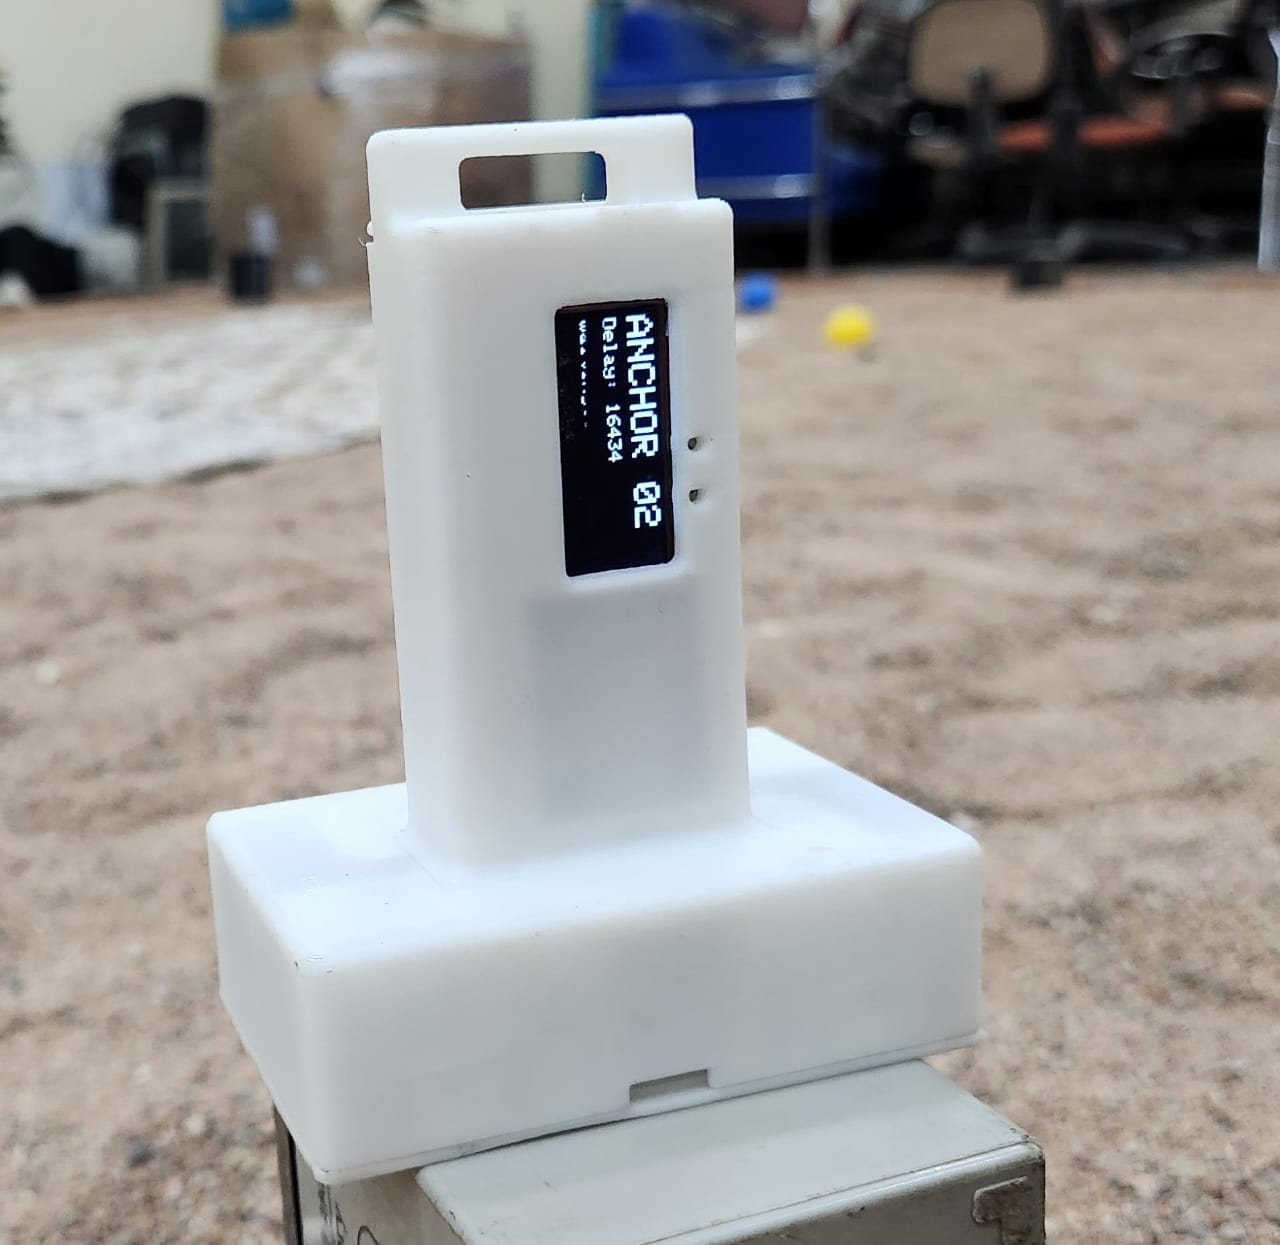
\includegraphics[width=\linewidth]{figures/anchor_unit.jpg}%
    }{%
      \fbox{\parbox{\linewidth}{\centering\vspace{1.6cm}
        \textit{[save anchor photo as figures/anchor\_unit.jpg]}
        \vspace{1.6cm}}}%
    }
  \end{minipage}\hfill
  \begin{minipage}{0.46\columnwidth}
    \centering
    \IfFileExists{figures/tag_unit.jpg}{%
      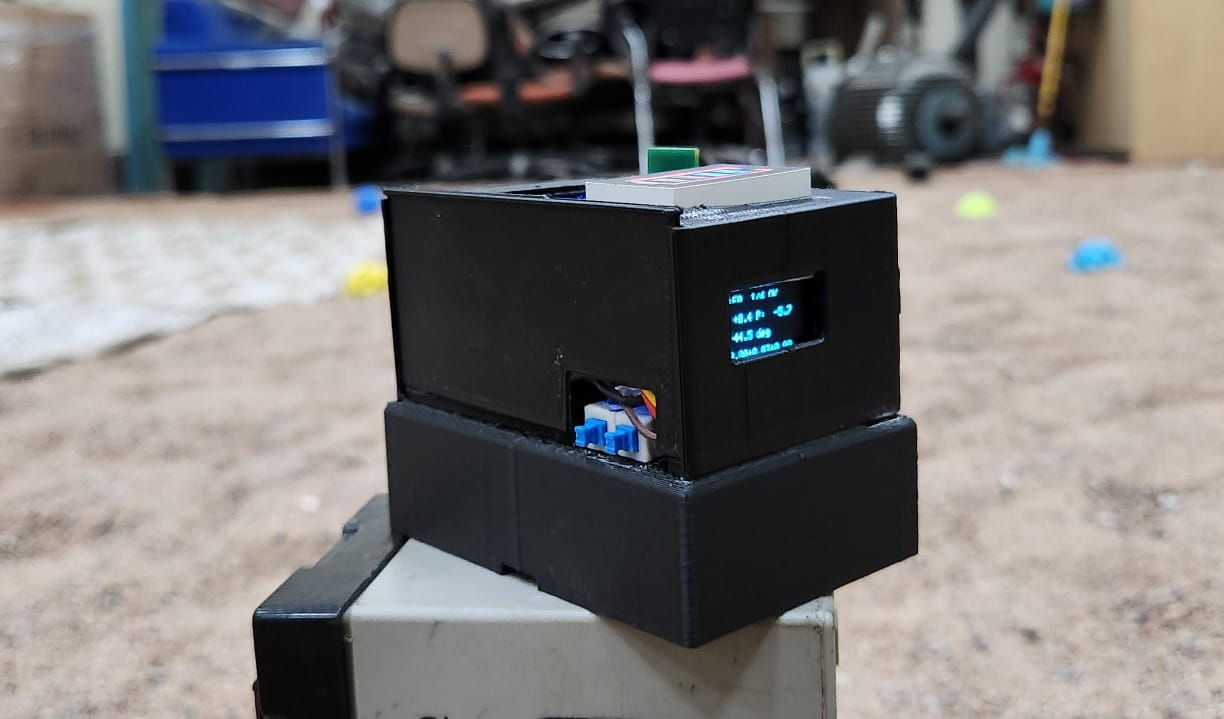
\includegraphics[width=\linewidth]{figures/tag_unit.jpg}%
    }{%
      \fbox{\parbox{\linewidth}{\centering\vspace{1.6cm}
        \textit{[save tag photo as figures/tag\_unit.jpg]}
        \vspace{1.6cm}}}%
    }
  \end{minipage}
  \caption{DUNE hardware units.
  \textit{Left}: Anchor node (Makerfabs ESP32 UWB Pro with Display, white enclosure)
  mounted on a stand; OLED shows node ID and calibrated antenna delay.
  \textit{Right}: Tag node (black enclosure) co-mounted with BNO085 IMU;
  OLED shows live range readings and heading output.}
  \label{fig:hw_units}
\end{figure}

Five anchors are deployed in the $5\,\text{m}\times5\,\text{m}$ sandbed:
anchors $A_1$--$A_4$ coplanar near the floor; anchor $A_5$ elevated at
$h_e \approx 1.0$\,m directly above $A_4$.
The elevation of $A_5$ makes $p_z$ observable by trilateration
(four coplanar anchors give a degenerate 3D geometry).
Two tags, Tag~1 (\texttt{0xF0}) and Tag~2 (\texttt{0xF1}), are mounted
rigidly on the rover chassis at separation $L = \SI{50}{\centi\metre}$.
Tag~1 carries the BNO085 9-DOF AHRS.

\begin{figure}[h]
  \centering
  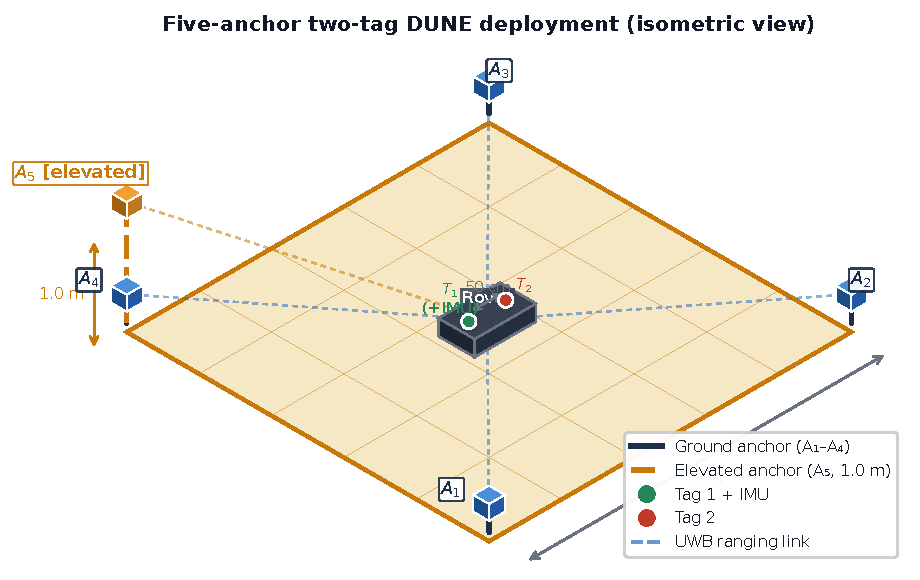
\includegraphics[width=\columnwidth]{figures/anchor_topology.pdf}
  \caption{Isometric view of the five-anchor two-tag DUNE deployment.
  Ground anchors $A_1$--$A_4$ at sandbed corners; anchor $A_5$ elevated
  at $1.0$\,m directly above $A_4$, making $p_z$ observable by 3D trilateration.
  The rover carries Tags $T_1$ (with BNO085 IMU) and $T_2$ at $L=50$\,cm baseline.}
  \label{fig:topology}
\end{figure}

\subsection{Full 6-DOF Pose Pipeline}
\label{sec:dual_tag_heading}

A single tag provides only 3D position.
Two tags at a rigid separation on the rover yield geometric yaw:
\begin{equation}
  \psi = \mathrm{atan2}\!\bigl(
    \hat{p}_{y,2} - \hat{p}_{y,1},\;
    \hat{p}_{x,2} - \hat{p}_{x,1}
  \bigr) + \psi_{\text{offset}},
  \label{eq:dual_tag_yaw}
\end{equation}
where $\psi_{\text{offset}}$ encodes the tag-to-rover-body alignment.
If each tag's 2D position error is $\sigma_p$, the expected yaw error is
\begin{equation}
  \sigma_\psi \approx \frac{\sqrt{2}\,\sigma_p}{L}
    = \frac{\sqrt{2} \times \todo{0.03}}{0.50} \approx \todo{4.8}\degree.
  \label{eq:yaw_accuracy}
\end{equation}

The complete 6-DOF pose is assembled from three sources:
\textbf{XYZ} from 3D trilateration with all 5 anchors (both tags independently);
\textbf{yaw $\psi$} from Eq.~\eqref{eq:dual_tag_yaw};
\textbf{roll $\phi$ and pitch $\theta$} from the BNO085 AHRS at
$\approx\SI{100}{\hertz}$.
A Singer-model EKF fuses UWB positions and IMU at the \SI{10}{\hertz} sweep
rate to produce the full output $(x,y,z,\phi,\theta,\psi)$.

\subsection{Firmware and Host Software}

\textbf{Host pipeline.}
All position computation runs on a host laptop; the rover MCU streams only
raw ranges (Fig.~\ref{fig:pipeline}).
Each sweep is processed as:
\begin{align*}
&\text{ranges}
 \xrightarrow{\text{Tier-2}} \text{corrected}
 \xrightarrow{\text{median}} \text{filtered}
 \xrightarrow{\text{NLOS}} \text{LM solve} \\
&\xrightarrow{\text{EKF}} \hat{\mathbf{x}}
 \xrightarrow{\text{EMA}} (x,y,z,\phi,\theta,\psi)
\end{align*}

\begin{figure}[h]
  \centering
  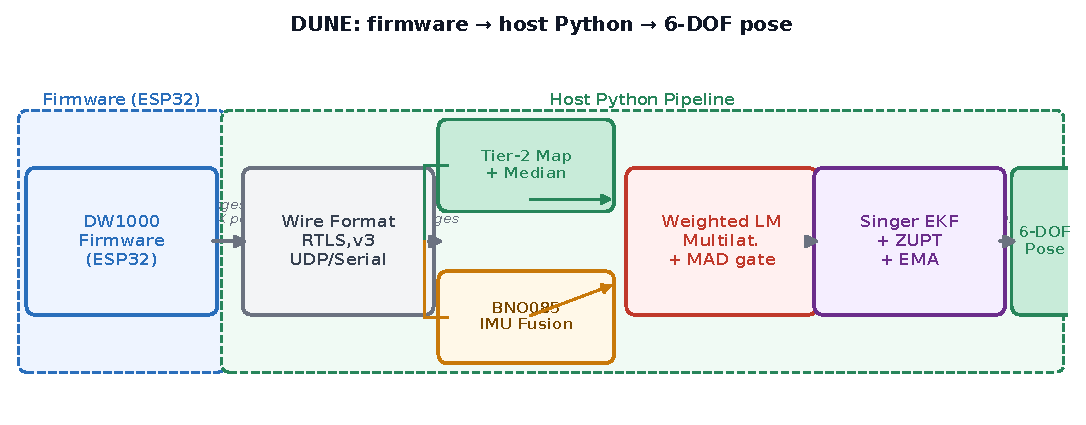
\includegraphics[width=\columnwidth]{figures/system_pipeline.pdf}
  \caption{DUNE system pipeline: DW1000 firmware streams raw ranges and NLOS
  power readings over Wi-Fi UDP; the Python host applies spatial corrections,
  NLOS-weighted trilateration, and Singer-EKF fusion to produce 6-DOF pose.}
  \label{fig:pipeline}
\end{figure}

\textbf{Wire format.}
The tag emits one ASCII line per sweep:
\begin{verbatim}
RTLS,v3,<t_ms>,<tag_id>,<n>,
  <id>,<d_mm>,<rx_dbm>,<fp_dbm>,<q>,...
  [,IMU,<status>,<qw>,<qx>,<qy>,<qz>,...]
\end{verbatim}
Fields \texttt{fp\_dbm} and \texttt{rx\_dbm} are the per-anchor NLOS inputs
(\S\ref{sec:nlos}).
Adding anchors or tags requires no firmware change.
